\chapter{Results}
\label{chap:results}

In this chapter the results of all experiments are presented. Every result is put into perspective and discussed. \\
Section \ref{sec:classification_results} shows the result of the classification experiments while Section \ref{sec:object_detection_results} shows the results of the object detection experiments with all subexperiments such as small data experiments and timing experiments. 

\section{Classification}
\label{sec:classification_results}

The network in combination with the scattering transform is able to classify all test data correctly with 100 percent accuracy after two episodes of training before it starts overfitting to the training data. In comparison, the network without the scattering transform achieves 99.65 percent accuracy after four episodes before it starts overfitting. This shows that the scattering transform is able to provide useful information, at least when presented with simple datasets as shown in Figure \ref{fig:toy_data_class_samples}. Further implications like a slightly better accuracy or a slightly faster convergence are potentially true, but cannot be concluded with high confidence from this single observations. This experiment gets its relevance for this paper by showing classification, a necessary condition for object detection, is fulfilled.

\section{Object Detection}
\label{sec:object_detection_results}
The results of the object detection experiments are presented in the following. First the baselines of the standard approach are established in Subsection \ref{subsec:baseline_SSD_results}. Then the experimental results of the sequential and parallel scattering approach are shown and discussed in Subsection \ref{subsec:sequential_scattering_results} and \ref{subsec:parallel_scattering_results} respectively. Lastly, Subsections \ref{subsec:small_data_results} and \ref{subsec:timing_evaluation_results} show the results of the small data and timing experiments respectively. 

\subsection{Baseline Performance of the SSD}
\label{subsec:baseline_SSD_results}

In this section the results of all the main experiments are presented. First the baselines that establish reasonable values for the use of batch norm and augmentations. Additionally, the baselines for comparison with the hybrid networks are determined. In the second subsection the results of the sequential scattering experiments are presented while the third subsection shows those of the parallel approach.

\subsubsection{Hyperparameterization and Baselines}

The average and standard deviation (std) of a given combination of variables can be found in Table \ref{table:baseline}. The coefficient of the GLM for \textit{augmentations} are positive and it is therefore used as a standard for future experiments. The p-value is 0.044 < 0.05 and we can therefore say it has a significant positive effect on the training. The coefficient for batch norm is also positive and is used in later experiments. Its p-value, however, is 0.79 > 0.05 and therefore we cannot assume that it has a significant positive effect. \textit{Pretraining} on ImageNet has a positive coefficient as well but no significant p-value with 0.41. Future experiments will still consider both possible values of \textit{pretrained} since interesting information about the network structure might be analyzed. On average the combination of \textit{augmentations}, no \textit{batchnorm} and \textit{pretrained} has the highest mean accuracy for all datasets. For PASCAL VOC an accuracy of 0.630 is achieved, for Kitti it is 0.125 and for the Toy data it is 0.792. These are the baselines to be compared with the results of the scattering experiments. The standard deviations show that the networks converge to somewhat similar functions even if their results deviate by some noise. Given that outliers were removed prior to the GLM fitting the standard deviations are only minor. 

\begin{table}[!htb]
	\centering
	\caption{Results of the baseline experiments. Mean and standard deviation are denoted for every combination of features that were measured. The results show that the combination of \textit{augmentations} and \textit{pretrained} true and \textit{batchnorm} false achieve the highest accuracy in all cases.}
	\begin{tabular}{lrrrrr}
		\toprule
		Dataset &  Augmentations &  Batchnorm &  Pretrained &   Mean &  Std\_dev \\
		\midrule
		VOC &              0 &          0 &           0 &  0.108 &    0.008 \\
		VOC &              0 &          0 &           1 &  0.363 &    0.055 \\
		VOC &              0 &          1 &           0 &  0.329 &    0.041 \\
		VOC &              0 &          1 &           1 &  0.341 &    0.017 \\
		VOC &              1 &          0 &           0 &  0.364 &    0.025 \\
		VOC &              1 &          0 &           1 &  \textbf{0.630} &    0.003 \\
		VOC &              1 &          1 &           0 &  0.568 &    0.002 \\
		VOC &              1 &          1 &           1 &  0.619 &    0.007 \\ \hdashline
		Kitti &              0 &          0 &           0 &  0.027 &    0.024 \\
		Kitti &              0 &          0 &           1 &  0.032 &    0.009 \\
		Kitti &              0 &          1 &           0 &  0.032 &    0.010 \\
		Kitti &              0 &          1 &           1 &  0.024 &    0.002 \\
		Kitti &              1 &          0 &           0 &  0.050 &    0.010 \\
		Kitti &              1 &          0 &           1 &  \textbf{0.125} &    0.011 \\
		Kitti &              1 &          1 &           0 &  0.116 &    0.012 \\
		Kitti &              1 &          1 &           1 &  0.113 &    0.010 \\ 
		\hdashline
		Toy\_data &              0 &          0 &           0 &  0.487 &    0.060 \\
		Toy\_data &              0 &          0 &           1 &  0.505 &    0.027 \\
		Toy\_data &              0 &          1 &           0 &  0.511 &    0.123 \\
		Toy\_data &              0 &          1 &           1 &  0.474 &    0.053 \\
		Toy\_data &              1 &          0 &           0 &  0.773 &    0.017 \\
		Toy\_data &              1 &          0 &           1 &  \textbf{0.792} &    0.049 \\
		Toy\_data &              1 &          1 &           0 &  0.613 &    0.128 \\
		Toy\_data &              1 &          1 &           1 &  0.710 &    0.058 \\
		\bottomrule
	\end{tabular}
	\label{table:baseline}
\end{table}

All results of the GLM can be found in the appendix in figure \ref{fig:GLM_baseline}. 


\subsubsection{Invariant toy data}

The results of the invariant toy data experiments with the standard architecture with \textit{augmentations} and \textit{batchnorm} set to true can be found in Table \ref{table:invariant_data}. All experiments have on average a slightly higher accuracy for the model without \textit{pretraining}. This is confirmed by the negative coefficient of the GLM that can be found in the appendix in Figure \ref{fig:GLM_invariances}. All other results of the GLM are in the same figure.  This seems plausible given that the invariances of geometric object have nothing to do with the patterns learned on real life objects from ImageNet. The networks are able to recognize objects with deformation with accuracy of 0.928. However the deformations are not that big which might be the primary reason for that result. Rotation and scale have and accuracy of 0.635 and 0.644 respectively. Translation has an accuracy of 0.002. This could be explained either by overfitting on the training set or a impossibility to generalize from the small number of training data. Overall it shows that the possibility to generalize is rather limited for a standard SSD network trained on a low number of training data points. All results of the GLM can be found in the appendix in Figure \ref{fig:GLM_invariances}. 

\begin{table}[!htb]
	\centering
	\caption{Results of the invariant toy data experiments. Mean and standard deviation are denoted for every combination of features that were measured. Pretraining on ImageNet decreases the average accuracy slightly.}
	\begin{tabular}{lrrr}
		\toprule
		Dataset &  Pretrained &   Mean &  Std\_dev \\
		\midrule
		Deformation\_data &           0 &  0.928 &    0.003 \\
		Deformation\_data &           1 &  0.896 &    0.026 \\\hdashline
		Rotation\_data &           0 &  0.635 &    0.010 \\
		Rotation\_data &           1 &  0.622 &    0.026 \\\hdashline
		Translation\_data &           0 &  0.001 &    0.001 \\
		Translation\_data &           1 &  0.002 &    0.001 \\\hdashline
		Scale\_data &           0 &  0.644 &    0.006 \\
		Scale\_data &           1 &  0.637 &    0.004 \\
		\bottomrule
	\end{tabular}
	\label{table:invariant_data}
\end{table}

\subsection{Sequential Scattering}
\label{subsec:sequential_scattering_results}

The results of the sequential scattering experiments with \textit{augmentations} and \textit{batchnorm} set true can be found in Table \ref{table:sequential_scattering_experiments}. \textit{Pretraining} on ImageNet does not make a significant difference for the resulting accuracy. The GLM in the appendix \ref{fig:GLM_sequential_scattering} even shows a negative sign of the responding coefficient. Hypothetically the pretrained weights could not only have learned the reoccurring contents of the images but also meaning that is independent of the representation of the data. Given the results of the experiments w.r.t. \textit{pretraining} this hypotheses can not be supported. \\
The explicit comparison to both other techniques will be done in the Comparison Subsection \ref{subsec:comparison_results} but two important differences stand out. The first is the major drop in accuracy of the PASCAL VOC dataset. While having 63 \% accuracy was reached with the standard SSD, only 43.2 \% was reached with sequential scattering. However, the standard setup was unable to identify objects after translation while the sequential scattering setup is able to achieve 85.7 \% accuracy thereby providing evidence for the equivariance given by the Scattering Transform. 

\begin{table}[!htb]
	\centering
	\caption{Results of the sequential scattering experiments. Mean and standard deviation of the accuracy are denoted for every combination of features that were measured. Pretraining on ImageNet does not add any benefit.}
	\begin{tabular}{lrrr}
		\toprule
		Dataset &  Pretrained &   Mean &  Std\_dev \\
		\midrule
		VOC &           0 &  0.399 &    0.004 \\
		VOC &           1 &  0.432 &    0.038 \\\hdashline
		Kitti &           0 &  0.110 &    0.001 \\
		Kitti &           1 &  0.077 &    0.003 \\\hdashline
		Toy\_data &           0 &  0.831 &    0.000 \\
		Toy\_data &           1 &  0.818 &    0.001 \\\hdashline
		Deformation\_data &           0 &  0.933 &    0.001 \\
		Deformation\_data &           1 &  0.929 &    0.001 \\\hdashline
		Rotation\_data &           0 &  0.590 &    0.014 \\
		Rotation\_data &           1 &  0.659 &    0.059 \\\hdashline
		Translation\_data &           0 &  0.857 &    0.000 \\
		Translation\_data &           1 &  0.767 &    0.127 \\\hdashline
		Scale\_data &           0 &  0.646 &    0.000 \\
		Scale\_data &           1 &  0.641 &    0.003 \\
		\bottomrule
	\end{tabular}
\label{table:sequential_scattering_experiments}
\end{table}

\subsection{Parallel Scattering}
\label{subsec:parallel_scattering_results}


The results for the parallel scattering experiments can be found in Table \ref{table:parallel_scattering_experiments}. Some of the standard deviations for the parallel scattering experiments are 0. This is the case because training the parallel network takes so much longer than the other networks that it was not possible to reproduce the experiments as often as the others in this paper. It can be seen that \textit{pretraining} on ImageNet has a positive impact on the results. This is also confirmed by the positive coefficient of the GLM that is reported in the appendix \ref{fig:GLM_parallel_scattering}. This also makes intuitive sense, given that much data is flowing through the path of the standard network. \\ Patterns similar to the sequential scattering approach arise, i.e. the accuracy on PASCAL VOC is significantly below the standard SSD but the drop of the translation data in the standard approach is not existent in the parallel scattering setup.

\begin{table}[!htb]
	\centering
	\caption{Results of the parallel scattering experiments. Mean and standard deviation of the accuracy are denoted for every combination of features that were measured. \textit{Pretraining} on ImageNet does improve accuracy.}
	\begin{tabular}{lrrr}
		\toprule
		Dataset &  Pretrained &   Mean &  Std\_dev \\
		\midrule
		VOC &           0 &  0.146 &    0.000 \\
		VOC &           1 &  0.476 &    0.000 \\\hdashline
		Kitti &           0 &  0.042 &    0.000 \\
		Kitti &           1 &  0.105 &    0.000 \\ \hdashline
		Toy\_data &           0 &  0.739 &    0.006 \\
		Toy\_data &           1 &  0.803 &    0.000 \\ \hdashline
		Deformation\_data &           0 &  0.900 &    0.000 \\
		Deformation\_data &           1 &  0.912 &    0.000 \\ \hdashline
		Rotation\_data &           0 &  0.684 &    0.007 \\
		Rotation\_data &           1 &  0.612 &    0.002 \\ \hdashline
		Translation\_data &           0 &  0.842 &    0.000 \\
		Translation\_data &           1 &  0.848 &    0.002 \\\hdashline
		Scale\_data &           0 &  0.641 &    0.001 \\
		Scale\_data &           1 &  0.640 &    0.001 \\
		\bottomrule
	\end{tabular}
\label{table:parallel_scattering_experiments}
\end{table}

\subsection{Comparison of the Techniques}
\label{subsec:comparison_results}

A final comparison between the best mean accuracies for all datasets and approaches can be seen numerically in Table \ref{table:comparison} and visually in Figure \ref{fig:comparison}. There are three key observations in the comparison. First, the results of the respective approaches differ in only two of the seven datasets. This is a positive result because it means that the Scattering Transform is a good alternative to the standard algorithms in object detection in most circumstances. Second, they differ in the results for PASCAL VOC where the standard approach outperforms both scattering approaches and they differ in the exact inverse direction for translation data. The first result is potentially due to the high background noise of natural images. The Scattering Transform is essentially an edge detector and the noise might produce a lot of edges in the scattering coefficients where none should be. This argument could also be used against the KITTI dataset, where no such effect is seen. Another hypotheses is that often objects in VOC images are behind each other or have high overlap, i.e. a human rider on the back of a horse. This is not given to a similar extend for the KITTI dataset. The Scattering Transform might have harder time to differentiate foreground/background relations since it mostly works on edge detection. In the case of translation data the standard approach is not general enough to learn the concept of object translation. The Scattering Transform, in contrast, already naturally contains prior knowledge in form of equivariance w.r.t. translation achieving significantly better results then the standard approach. The third observation is the comparison of the scattering techniques between each other. Figure \ref{fig:comparison} shows that the respective lines of sequential and parallel scattering are nearly identical. This either means that the concatenation of the scattering results introduces an upper bound to the performance of the standard path or that the concatenation is done in a way in which the scattering results dominate the normal pathway. The last possibility is more likely in the context of this paper since the second concatenation of the scattering transform merges 243 scattering filters with 128 feature maps from the standard CNN path. At this point the information from the standard path ways might be ignored by later layers given their numerical minority. Future experiments could contain a concatenation with less scattering filters. 

\begin{table}[!htb]
	\centering
	\caption{Comparison between the standard SSD, sequential scattering and parallel scattering. For each method the best mean accuracy for all datasets is reported and compared. The standard SSD outperforms both others on VOC. The inverse happens in translation data.}
	\begin{tabular}{lrrr}
		\toprule
		{} &  Standard SSD &  Sequential Scattering &  Parallel Scattering \\
		\midrule
		Kitti            &         0.125 &                  0.110 &               0.1048 \\
		VOC              &         0.630 &                  0.432 &               0.4760 \\
		Toy\_data         &         0.792 &                  0.831 &               0.8030 \\
		Deformation\_data &         0.928 &                  0.933 &               0.9120 \\
		Rotation\_data    &         0.635 &                  0.659 &               0.6840 \\
		Translation\_data &         0.002 &                  0.857 &               0.8480 \\
		Scale\_data       &         0.644 &                  0.646 &               0.6400 \\
		\bottomrule
	\end{tabular}
	\label{table:comparison}
\end{table}

\begin{figure}[!htb]
	\centering
	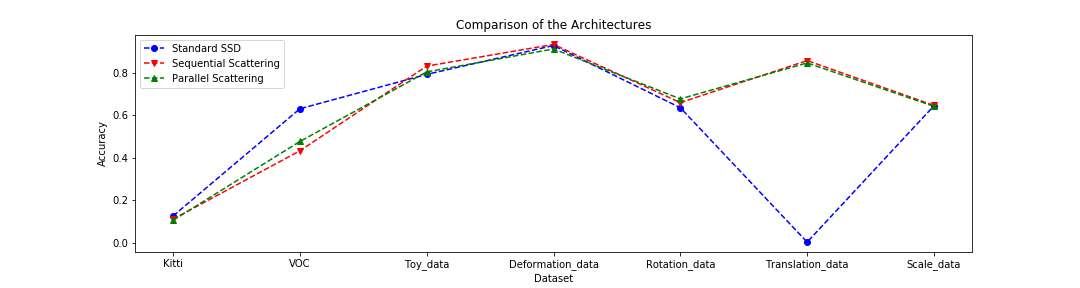
\includegraphics[width=\textwidth]{images/comparison.png}
	\caption{Comparison between the standard SSD, sequential scattering and parallel scattering. For each method the best mean accuracy for all datasets is reported and compared. The standard SSD outperforms both others on VOC. The inverse happens in translation data.}
	\label{fig:comparison}
\end{figure}

\subsection{Small Data Experiments}
\label{subsec:small_data_results}

The results of the small data experiments can be found in table \ref{table:small_data_experiments}. On the small toy dataset the sequential scattering outperforms both the standard and the parallel scattering network significantly with 0.759 to 0.630 and 0.411 for 25k epochs and 0.121 to 0.043 and 0.003 for 5k epochs. In the case of the PASCAL VOC dataset the standard SSD outperforms both others with 0.317 to 0.053 and 0.013 for 25k epochs and 0.025 to 0.011 and 0.004 for 5k epochs. The conclusions from this are twofold: a) The sequential scattering setup is useful in specific use cases while having problems with very noisy and unstructured datasets such as VOC and b) The parallel scattering approach (at least with the setup used in this paper) does not really yield the expected results. Instead of providing the best of both techniques the parallel scattering gets outperformed on both datasets. All results of the GLM can be found in the appendix in Figure \ref{fig:GLM_small_data}. 


\begin{table}[!htb]
	\centering
	\caption{Results of the small data experiments. Mean and standard deviation of the accuracy are denoted for every combination of features that were measured.}
	\begin{tabular}{lllrr}
		\toprule
		Dataset & epochs &           network type &   Mean &  Std\_dev \\
		\midrule
		Toy\_data\_small &    25k &               standard &  0.630 &    0.008 \\
		Toy\_data\_small &    25k &  sequential\_scattering &  0.759 &    0.004 \\
		Toy\_data\_small &    25k &    parallel\_scattering &  0.411 &    0.012 \\
		Toy\_data\_small &     5k &               standard &  0.043 &    0.007 \\
		Toy\_data\_small &     5k &  sequential\_scattering &  0.121 &    0.027 \\
		Toy\_data\_small &     5k &    parallel\_scattering &  0.003 &    0.001 \\
		\hdashline
		VOC &    25k &               standard &  0.317 &    0.011 \\
		VOC &    25k &  sequential\_scattering &  0.053 &    0.006 \\
		VOC &    25k &    parallel\_scattering &  0.013 &    0.001 \\
		VOC &     5k &               standard &  0.025 &    0.001 \\
		VOC &     5k &  sequential\_scattering &  0.011 &    0.007 \\
		VOC &     5k &    parallel\_scattering &  0.004 &    0.000 \\
		\bottomrule
	\end{tabular}
	\label{table:small_data_experiments}
\end{table}

\subsection{Timing Evaluation}
\label{subsec:timing_evaluation_results}

The results of the timing evaluation can be found in Table \ref{table:timing_evaluation}. The sequential scattering SSD setup is the fastest with an average of 0.178 seconds per forward pass followed by the normal SSD setup with 0.236 seconds. Both are far ahead of the parallel scattering setup with 1.499 seconds per forward pass. The standard deviations are very small in all cases as a result of the deterministic nature of all three methods. The timing is not compared to other network setups, i.e. a ResNet instead of a VGG, since the scattering approach is easily transferable to other networks and relative results are therefore the only relevant ones. \\
There are two conclusions to be drawn from these results. First, the sequential scattering is slightly faster than the normal SSD and therefore could replace it in specific niche tasks when both have the same accuracy. Second, the parallel scattering approach is slower by a factor of 6-9 and is therefore only justified either when time is no constraint (e.g. offline applications) or when the accuracy of the parallel approach far outperforms the other two. The reason for the parallel approach taking so much longer than the other two is the calculation of second order coefficients. If this is left out. This approach should only be marginally slower.

\begin{table}[!htb]
	\centering
	\caption{Mean and standard deviation (std.) of 100 runs of the timing evaluation for the normal SSD, the sequential and the parallel scattering SSD are shown. Means are reported in seconds. The sequential scattering is faster than the standard approach. Both are significantly faster than the parallel scattering.}
	\begin{tabular}{lcc}
		\toprule
		network type & mean & std. \\
		\midrule
		normal SSD & 0.236 & 0.004 \\
		sequential scattering & 0.178 & 0.004 \\
		parallel scattering & 1.499 & 0.002 \\
		\bottomrule
	\end{tabular}
	\label{table:timing_evaluation}
\end{table}
